%=========================================
% 	   Fallbeispiel     		 =
%=========================================
\chapter{Fallbeispiel}
In diesem Kapitel stellen wir, eine anhand eines selbst ausgedachten Anwendungsfalls, Cloud-Native Architektur vor, die wir prototypisch implementiert haben.

\section{Beschreibung}
Im Rahmen des Beispiels, haben wir eine Cloud-Native Architekturn für ein Chatprogramm (ChatApp) entworfen. Die Applikation soll drei Funktionen besitzen. Benutzer sollen sich registrieren können, Benutzer sollen sich ein-und ausloggen können und Benutzer sollen Nachrichten an andere Benutzer schreiben können. Im folgenden sind alle funktionalen und nichtfunktionalen Anforderungen aufgeführt.


\section{Anforderungen}
\subsection{Nichtfunktionale Anforderungen}
1. Skalierbarkeit
Das System muss mit einer großen Zahl von Benutzern, die das System gleichzeit verwenden, umgehen können.

2. Verfügbarkeit
Das System muss zu jeder Zeit verfügbar sein.

3. Sicherheit
Das System muss Berechtigungen überprüfen können (z.B. darf Benutzer X die Nachrichten lesen) und das System sollte sich gegen übliche Cyberangriffe (z.B. DDoS) schützen können.

4. Änderbarkeit/Erweiterbarkeit
Das System muss es zulassen, dass weitere Komponenten (z.B. Hochladen von Bildern und Videos) einfach hinzugefügt werden können.

\subsection{Funktionale Anforderungen}
1. Registierung
Ein Benutzer kann sich mit seiner E-Mail Adresse und einem Passwort im System registieren.

2. Ein- und Ausloggen
Ein Benutzer kann sich mit seiner E-Mail Adresse und seinem Passwort im System anmelden und danach die Funkionen nutzen bis er sich abmeldet.

3. Nachrichten schreiben/lesen
Ein Benutzer kann Nachrichten an andere Benutzer senden und Nachrichten, die an ihn gesendet worden sind, abrufen.


Im nächsten Abschnitt stellen wir die von uns entworfene Architektur vor und erläutern die wichtigsten Merkmale. 

\begin{figure}[bth] 
	\centering
	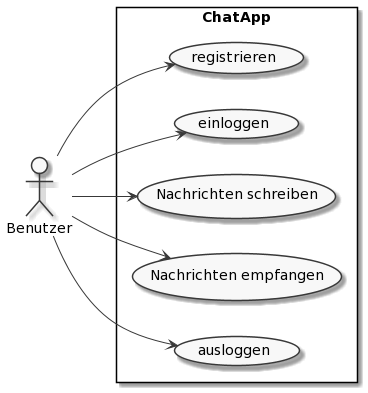
\includegraphics[width=0.6\textwidth]{Graphics/Usecase-Diagramm.png}
	\caption{Use-Case Diagramm}
\end{figure}

\section{Architekturentwurf}

\subsection{Übersicht}
Wie in Abbildung xx zu sehen ist besteht die Architektur aus einem Client mit graphischer Oberfläche (UI) einem API-Gateway, das alle Anfragen von Clienten empfängt und drei Microservices mit je einer eigenen Datenbank, die die Hauptfunktionalitäten des Systems implementieren.

\subsection{Microservices}
Jede Funktion aus den Anforderungen korrespondiert mit einem Microservice. Die Aufteilung der Microservices ergibt sich aus der Annahme, dass die Funkionalitäten, die sie bereitstellen unterschiedlich oft genutzt werden: Anzahl der Registrierungen < Anzahl Login/Logout < Anzahl der geschriebenen Nachrichten/Abruf von Nachrichten). Daraus gewinnen wir eine individuelle Skalierbarkeit der Funktionen, sodass die Architektur für eine hohe Anzahl von Benutzern geeignet ist.

verfügbarkeit
ändrebarkeit
sicherheit

kommunikation
wahl der technologie

\subsection{API-Gateway}
Das API-Gateway schottet die Microservices ab. Das bedeutet, dass alle Anfragen vom Clienten nur an das API-Gateway gesendet werden und niemals direkt an die Microservices. Das Gateway leitet dann die Anfrage an den entsprechenden Mircoservice weiter und sendet dessen Antwort wieder an den Clienten. Die Abschottung hat mehrere Vorteile. Sicherheitsrelevante Aspekte wie z.B. DDOS-Protection oder der Schutz vor unbefugtem Zugriff (von Adressen, die nicht zum Client gehören) können auf das API-Gateway verlagert werden und müssen daher nicht in jedem Microservice implementiert werden.
Des Weiteren erfüllt das API-Gateway die Rolle eines Load-Balancers, der die Anfragen auf verschiedene Instanzen von Microservices verteilen kann. 

änderbarkeit

\subsection{Client}
Mithilfe des Clients können Anfragen an das System, genauer gesagt das API-Gateway, gesendet werden. Er enthält keine Funktionalitäten und dient lediglich zum Abrufen und Darstellen von Inhalten.


\subsection{Kommunikation}
Die Komponenten des Systems kommunizieren über Netzwerktechnologien miteinander. vorteile davon TODO

\begin{figure}[bth] 
	\centering
	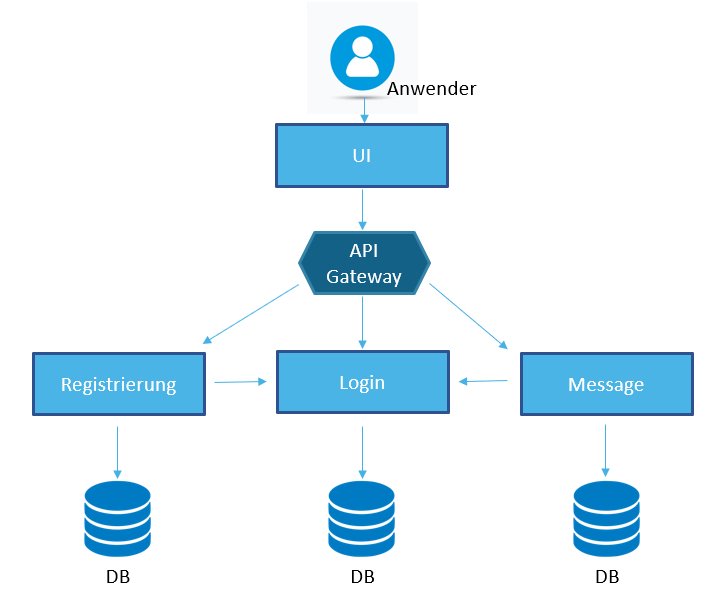
\includegraphics[width=0.6\textwidth]{Graphics/Architekturentwurf.png}
	\caption{Architekturentwurf}
\end{figure}

\begin{figure}[bth] 
	\centering
	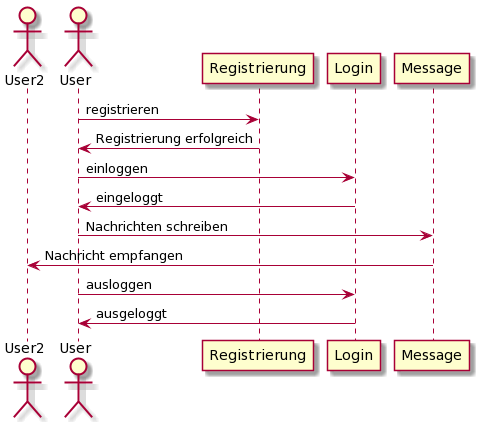
\includegraphics[width=0.6\textwidth]{Graphics/Sequenzdiagramm.png}
	\caption{Sequenzdiagramm}
\end{figure}

\section{Implementierung des Prototyps}

In diesem Kapitel stellen wir unsere prototypische Implementierug vor. Das gesamte System ist in fünf Teile aufgeteilt (UI, API-Gateway, Registration-Microservice, Login-Microservice und Message-Microservice), wobei jeder Teil einem unabhängigem Projekt entspricht, aus welchem jeweils ein eigenständig ausführbares Programm ensteht.

\subsection{UI}

\subsection{API-Gateway}
Das API-Gateway ist mit Java und Maven als Build-Management-Tool implementiert. Es stellt mehrere HTTP Endpunkte zur Verfügung, an die Nachrichten gesendet werden können, die es dann an die Microvervices weiterleitet. Für das Gateway sind die Microservices ebenfalls HTTP Endpunkte.
Das Loadbalancing ist für den Message-Microservice implementiert. Dabei kennt das API-Gateway zwei verschiedene Endpunkte unter denen jeweils eine Instanz des Message-Microservices auf Anfragen hört. Bekommt das Gateway eine Anfrage für den Message-Microservice wird abwechselnd eine der beiden Instanzen ausgewählt, an welche die Anfrage weitergeleitet wird.

\subsection{Registration-Microservice}

\subsection{Login-Microservice}

\subsection{Message-Microservice}